\section{Architecture}
For building up a network architecture two methods are predominantly used in games; the peer-to-Peer and the client-server based architecture.

\subsection{Client-Server}\cite{networkingTypes}
The Client-Server model consist of clients and a server as shown in Figure \ref{fig:server_client}. 

\begin{figure}[H]
\centering
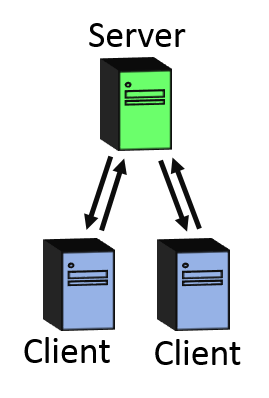
\includegraphics[scale=1]{figures/network/server_client}
\caption{An illustration of the server/client model.}
\label{fig:server_client}
\end{figure}

In the traditional client-server model, the server handles all computations and the results are then communicated to the clients.
Clients act as \textit{dumb terminals} that redirect input from the user of the client to the server.
The server computes the next frame or the simulation and sends the information back to the clients which then updates their games state accordingly.


\subsection{Peer-to-Peer}\cite{networkingTypes}
The peer-to-peer model consists only of peers with no dedicated server.
In this model, peers communicate directly with each other as shown in Figure \ref{fig:peer_peer}

\begin{figure}[H]
\centering
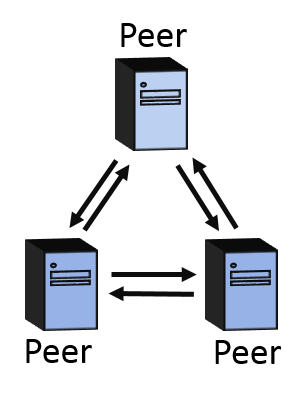
\includegraphics[scale=1]{figures/network/peer_peer}
\caption{An illustration of the Peer-to-peer model.}
\label{fig:peer_peer}
\end{figure}

Peer-to-Peer (\textit{P2P}) network model in games ideally consists of turns.
Each turn, peers gathers input from each peer who then individually executes all the commands on each machine.
The purpose of this is that, given a deterministic game, the game that are running on each individual computer will be running the exact same code.
Therefore given the game is deterministic the game state will be exactly the same on each computer.

\subsection{Choosing an architecture}
The client-server architecture is popular in games because it does not limit the update rate of the game based on the connection of the slowest player, but instead only based on the connection of the server.
Peer-to-peer becomes more complex as more peers join the game, while client-server does not.
Thus we choose the client-server architecture.
